\section{Mô tả thiết kế}

\subsection{Kiến trúc tổng thể}
Thiết kế bao gồm các module chính:
\begin{itemize}[leftmargin=1.2cm]
    \item Processor Interface
    \item I2C Master Control FSM
    \item I2C Bus Control FSM
    \item Clock Generator \& Synchronizer
    \item Tx Data FSM \& Rx Data FSM
    \item Start/Stop detect \& generate logic
    \item Acknowledge logic
\end{itemize}

\begin{figure}[H]
    \centering
    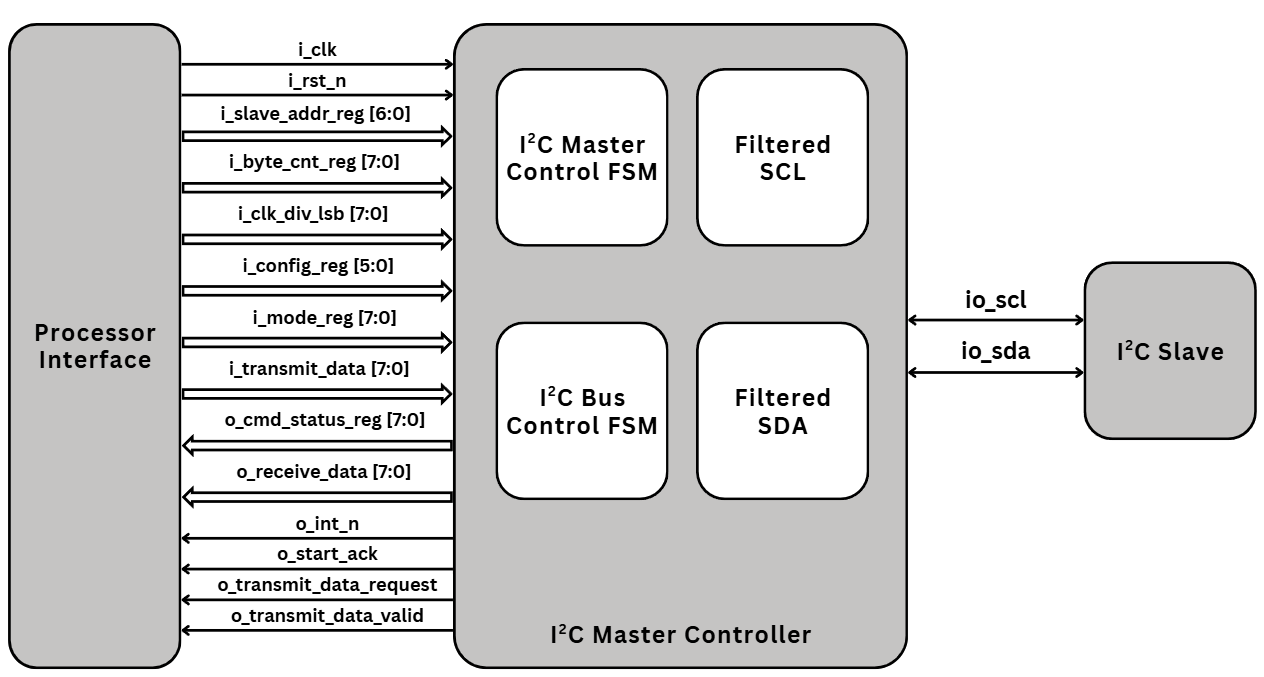
\includegraphics[width=0.92\textwidth,keepaspectratio]{figures/i2c_from_docx/top_module_block_diagram.png}
    \caption{Sơ đồ khối I2C Master Controller (top module)}
    \label{fig:block}
\end{figure}

Hình \ref{fig:block} thể hiện ranh giới giữa \textbf{Processor Interface} và lõi \textbf{I\textsuperscript{2}C Master Controller}. Phía CPU cấu hình các thanh ghi:
\begin{itemize}[leftmargin=1.2cm]
    \item \texttt{i\_slave\_addr\_reg[6:0]} (địa chỉ 7-bit), \texttt{i\_byte\_cnt\_reg[7:0]} (số byte),
    \item \texttt{i\_clk\_div\_lsb[7:0]} và \texttt{i\_mode\_reg[7:0]} (chọn tốc độ / mode),
    \item \texttt{i\_config\_reg[5:0]} (START/interrupt/abort/reset), \texttt{i\_transmit\_data[7:0]} (byte TX).
\end{itemize}

Lõi master xuất trạng thái và handshake về CPU: \texttt{o\_cmd\_status\_reg[7:0]}, \texttt{o\_receive\_data[7:0]}, \texttt{o\_int\_n}, \texttt{o\_start\_ack}, \texttt{o\_transmit\_data\_request}, \texttt{o\_transmit\_data\_valid}.

Bên trong controller có hai FSM chính:
\begin{itemize}[leftmargin=1.2cm]
    \item \textbf{I\textsuperscript{2}C Master Control FSM}: điều phối giao dịch ở mức byte.
    \item \textbf{I\textsuperscript{2}C Bus Control FSM}: điều khiển timing bus ở mức bit và tạo/nhận START/STOP/ACK.
\end{itemize}

Hai khối \textbf{Filtered SCL} và \textbf{Filtered SDA} là lớp đệm/lọc tín hiệu pad, nối ra bus \texttt{io\_scl} và \texttt{io\_sda} (open-drain) sang \textbf{I\textsuperscript{2}C Slave}.

\subsection{Mô tả các thanh ghi}
\begin{table}[H]
    \centering
    \caption{Register Description}
    \label{tab:reg}
    \begin{tabularx}{\textwidth}{|l|X|}
        \hline
        \textbf{Thanh ghi} & \textbf{Chức năng} \\
        \hline
        \texttt{i\_slave\_addr\_reg} & Địa chỉ 7-bit của slave. \\
        \hline
        \texttt{i\_byte\_cnt\_reg} & Số byte cần truyền/nhận. \\
        \hline
        \texttt{i\_clk\_div\_lsb} + \texttt{i\_mode\_reg[2:0]} & Bộ chia clock tạo SCL. \\
        \hline
        \texttt{i\_config\_reg} & Gồm các bit START, INT\_CLR, TX\_IE, RX\_IE, ABORT, RESET. \\
        \hline
        \texttt{o\_cmd\_status\_reg} & TX\_DONE, RX\_DONE, TX\_ERR, RX\_ERR, ABORT\_ACK, I2C\_BUSY. \\
        \hline
    \end{tabularx}
\end{table}

